\documentclass[12pt,spanish]{article}
\usepackage[utf8]{inputenc}
\usepackage{babel}
\usepackage{listings}
\usepackage{mathpazo}
\usepackage{enumitem}
\usepackage{courier}
\usepackage{textcomp}
\usepackage{xcolor}
\usepackage{parskip}
\usepackage{fullpage}
\usepackage{graphicx}

\newcommand{\onelinerule}{\rule[2.3ex]{0pt}{0pt}}
\newcommand{\twolinerule}{\rule[6.2ex]{0pt}{0pt}}
\newcommand{\respuesta}{\framebox[\textwidth]{\twolinerule}}
\newcommand{\nombre}{%
  \begin{tikzpicture}[xscale=.4,yscale=.7]
    \draw (0, 0) rectangle (22, 1);
  \end{tikzpicture}%
}
%\newcommand{\rol}   {\framebox[0.3\textwidth]{\onelinerule}}
\newcommand{\rol}{%
  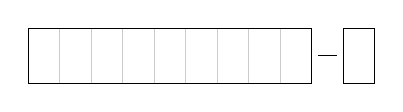
\begin{tikzpicture}[xscale=.4,yscale=.7]
    \draw[gray!40] ( 0, 0) grid      ( 9, 1);
    \draw          ( 0, 0) rectangle ( 9, 1);
    \draw          (10, 0) rectangle (11, 1);
    \draw (9 + .2, .5) -- (10 - .2, .5);
  \end{tikzpicture}%
}
\newcommand{\li}{\lstinline}
\newcommand{\pond}[1]{[{\small\textbf{#1\%}}]}

\lstdefinelanguage{py}{%
  classoffset=0,%
    morekeywords={%
      False,class,finally,is,return,None,continue,for,lambda,try,%
      True,def,from,nonlocal,while,and,del,global,not,with,print,%
      as,elif,if,or,yield,assert,else,import,pass,break,except,in,raise},%
    keywordstyle=\color{black!80}\bfseries,%
  classoffset=1,
    morekeywords={int,float,str,abs,len,raw_input,exit,range,min,max,%
      set,dict,tuple,list,bool,complex,round,sum,all,any,zip,map,filter,%
      sorted,reversed,dir,file,frozenset,open,%
      array,zeros,ones,arange,linspace,eye,diag,dot},
    keywordstyle=\color{black!50}\bfseries,%
  classoffset=0,%
  sensitive=true,%
  morecomment=[l]\#,%
  morestring=[b]',%
  morestring=[b]",%
  stringstyle=\em,%
}

\lstdefinelanguage{testcase}{%
  moredelim=[is][\bfseries]{`}{`},%
  backgroundcolor=\color{gray!20},%
}

\lstdefinelanguage{file}{%
  frame=single,%
  backgroundcolor=\color{white},%
}

\lstset{language=py}
\lstset{basicstyle=\ttfamily}
\lstset{columns=fixed}
\lstset{upquote=true}
\lstset{showstringspaces=false}
\lstset{rangeprefix=\#\ }
\lstset{includerangemarker=false}

\newlist{certamen}{enumerate}{1}
\setlist[certamen]{%
  label=\arabic*.,
  font=\LARGE\bfseries,%
  labelindent=-.5in,%
  leftmargin=0pt,%
  labelsep=1em%
}



\lstset{language=file,frame=single}

\begin{document}
  \thispagestyle{empty}
  \section*{Miércoles 14 de noviembre}

  El profesor Rogelio Bombal desea publicar una página web
  con los cumpleaños de los alumnos de Programística.

  Escriba el programa \texttt{cumples.py},
  que genere el archivo \texttt{cumples.html}.
  El contenido de este archivo debe seguir la estructura
  del ejemplo de más abajo.
  (Por limitaciones de espacio,
  aquí aparecen sólo los cumpleaños de los dos primeros meses.
  Su programa debe incluírlos todos).

  \begin{minipage}[T]{.40\textwidth}
    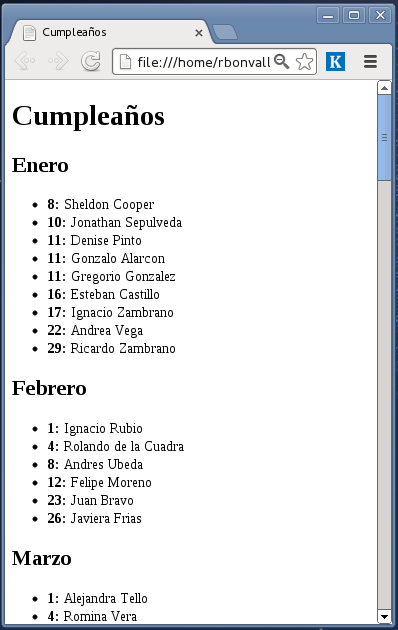
\includegraphics[width=\textwidth]{cumples.png}
  \end{minipage}
  \hfill
  \begin{minipage}[T]{.55\textwidth}
    Archivo \texttt{cumples.html}:
    \lstinputlisting[basicstyle=\small\ttfamily]{ejemplo.html}
  \end{minipage}

  \newpage

  \emph{(Opcional, sin nota).}
  Modifique su programa para que
  las personas que tienen cumpleaños el mismo día
  sean mostrados en la misma línea:

  \lstinputlisting[basicstyle=\small\ttfamily]{ejemplo-opcional.html}

  Los nombres deben aparecer separados por comas,
  excepto antes del último,
  que debe estar precedido por «y».

  \emph{(Opcional, sin nota).}
  Modifique su programa para que el nombre de cada persona
  sea un enlace para enviarle un mail.
  Para esto, el nombre debe ser escrito en el archivo
  como en el siguiente ejemplo:
  \begin{lstlisting}
<a href="mailto:a.vega@uvxyz.cl">Andrea Vega</a>
  \end{lstlisting}

\end{document}

